\chapter{Cluster analysis}
\label{clustan}

Cluster ``analysis'' describes a range of algorithms for investigating structure in data, the main interest is in finding groups of objects who are more alike.  A large number of books are dedicated to this one subject, for example \cite{Kaufman+Rousseeuw:1989,Everitt+etal:2001,Gordon:1999}, the former book supporting some rather interesting code that has been ported to \R (the S-PLUS version is described in  \cite{Struyf+etal:1997}).   It may be worth noting that some multivariate authors do not cover it at all \cite{Flury:1997} preferring a formulation based upon mixture models, and [page 316] \cite{Venables+Ripley:2002} indicate a preference for using visualisation methods for finding such structure in data.  Whilst cluster analysis is most often directed towards finding subsets of individuals that are more alike than other subsets, it is worth noting that variable clustering is also possible.   The heatmap in figure \ref{heatmap} has a dendrogram for both individuals and variables.

\singlespacing
\begin{verbatim}
x  <- as.matrix(mtcars)
rc <- rainbow(nrow(x), start=0, end=.3)
cc <- rainbow(ncol(x), start=0, end=.3)
hv <- heatmap(x, col = cm.colors(256), scale="column",
     RowSideColors = rc, ColSideColors = cc, margin=c(5,10),
     xlab = "specification variables", ylab= "Car Models",
     main = "Heatmap of mtcars data")
\end{verbatim}
\onehalfspacing

\begin{figure}
\begin{center}
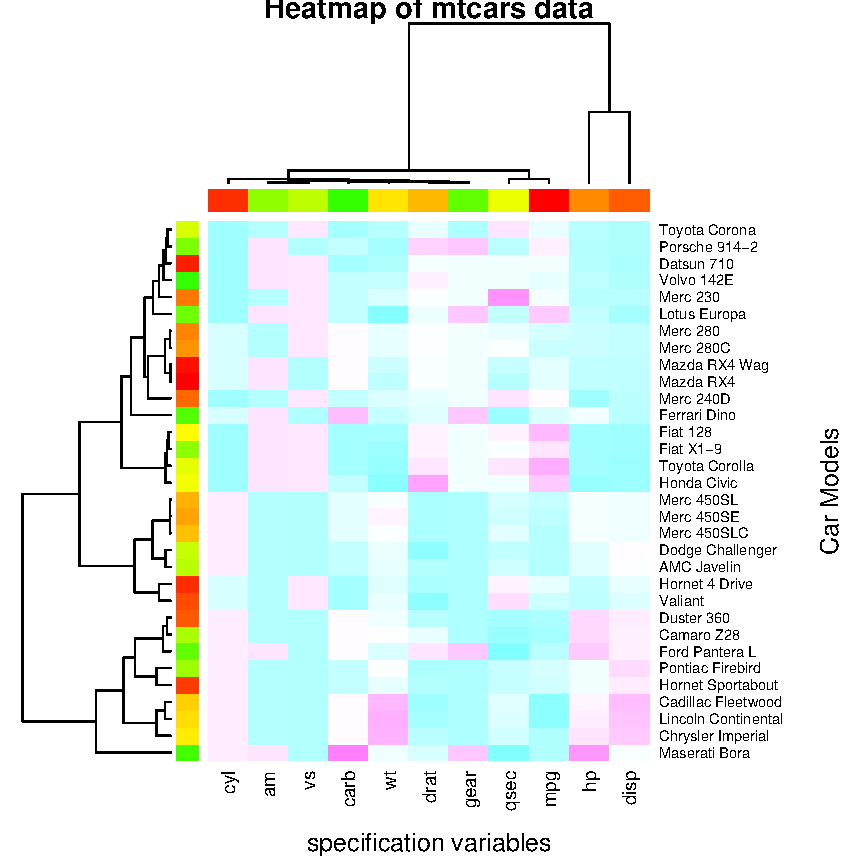
\includegraphics[width = 0.7\textwidth]{images/heatmap}
\caption{Heatmap of \texttt{mtcars} data; variables scaled in columns}
\label{heatmap}
\end{center}
\end{figure}

Modern computing facilities have widened the possibilities for visualisation considerable (both in terms of linked displays as well as the ability to numerically optimise various projection criteria).   However, when investigating the results of any scaling or projection methods there may still be interesting structures within the data.   The interest in cluster analysis lies in finding groups within the data.   When the objects within a group are very similar this can be described as internal cohesion (or homogeneity), when they is a large dissimilarity between groups this can be referred to as external separation (or isolation).   Where we have internal cohesion and external separation, one usually refers to the situation as ``clustering''. If the objects have been more-or-less
aribtrarily divided into groups we could refer to this as ``dissection''.
Clustering and dissection may both the useful in different
contexts (e.g. taxonomy and market research).   One attempt to illustrate this concept is given in figure \ref{partclust}.

%par(mfrow = c(1,2))

%x <- rbind(mvrnorm(20, c(0,-1), sigma), mvrnorm(20, c(5,4), sigma), mvrnorm(20, c(-5,4), sigma))
%plot(x, pch = 16, main = "Clustering", xlab = expression(x[1]), ylab = expression(x[2]) )
%lines(c(0,-6), c(4,-2))
%lines(c(0,0), c(4,7))
%lines(c(0,6), c(4,-1.4))
 
%x <- mvrnorm(60, c(0,4), sigma)
%plot(x, pch = 16, main = "Partitioning", xlab = expression(x[1]), ylab = expression(x[2]) )
%lines(c(0,-6), c(4,-2))
%lines(c(0,0), c(4,7))
%lines(c(0,6), c(4,-1.4))


\begin{figure}
\begin{center}
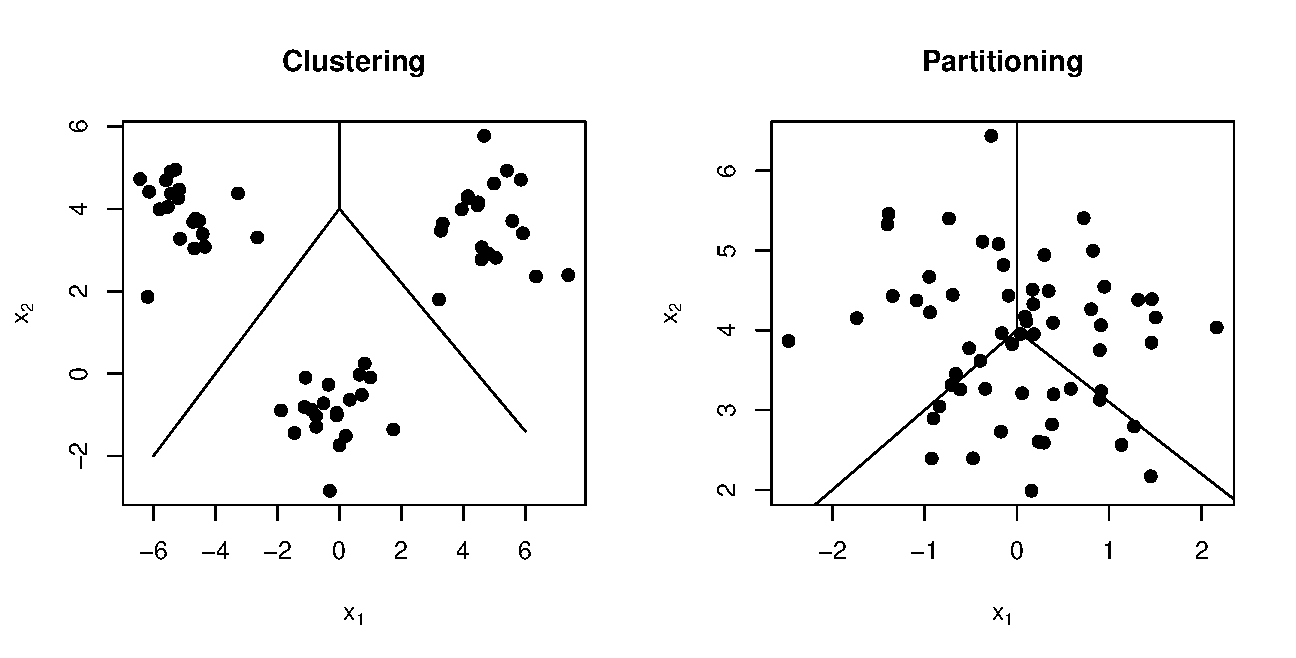
\includegraphics[width = 0.7\textwidth]{images/partclust}
\caption{Artificial data suggesting a difference between ``clustering'' and ``dissecting''}
\label{partclust}
\end{center}
\end{figure}


There are a wide range of algorithms that have been developed to investigate clustering within data.   These can be considered in a number of ways:

\begin{itemize}
\item Hierarchical Methods
  \begin{itemize}
  \item Agglomerative clustering (\verb+hclust()+, \verb+agnes()+)
  \item Divisive clustering (\verb+diana()+, \verb+mona()+)
  \end{itemize}
\item Partitioning methods (\verb+kmeans()+, \verb+pam()+, \verb+clara()+)
\end{itemize}


Hierarchical clustering provides a set of clusterings, either for $k = n, \ldots, 2$ (agglomerative) or $k = 2, \ldots, l$ (divisive).   The clustering is represented in a dendrogram and can be cut at arbitrary heights to give a fixed number of clusters.   It perhaps has a logical interpretation in numerical taxonomy.  Partitioning methods usually work by assuming a pre-determined number of clusters $k$ (although it is obviously possible to explore solutions over a range of values of $k$).   As [page 379] \cite{Seber:1984} points out, the number ofways $S_{k,n}$ of partitioning $n$ objects into $k$ groups, given by:
\begin{displaymath}
S_{k,n} = \frac{1}{k!} \sum_{j=1}^{k} \left( \begin{array}{c}k \\ j \end{array} \right) (-1)^{k-j} j^{n} \approx_{n \to \infty} \frac{k^{n}}{k!}
\end{displaymath} 
is a second type Stirling number, and where $k$ is not specified we have $\sum_{k=1}^{K} S_{k,n}$ partitions.   

For $n= 50$ and $k=2$ this is in the order of $6 \times 10^{29}$

\section{Introduction to agglomerative hierarchical cluster analysis}

Hierarchical cluster analysis finds representations that obey the ultrametric inequality.

\begin{displaymath}
d(x_{ij}, x_{ik}) \leq max(d(x_{ij}, x_{il}) d(x_{il}, x_{ik}) )
\end{displaymath}

We will work through three conventional examples of cluster analysis manually before considering an \R implementation in more detail.   For the sake of the demonstations, consider the following distance matrix:

\begin{tabular}{r|ccccc}
 & a & b & c & d & e\\
\hline
a & 0  &   &   &   &\\
b & 2  & 0 &   &   &\\
c & 6  & 5 & 0 &   & \\
d & 10 & 9 & 4 & 0 &  \\
e & 9  & 8 & 5 & 3 & 0\\
\end{tabular}

Initially, each individual is put in its own cluster.   Subsequently, at each stage individuals are joined to other individuals to form clusters, and the distance measure between a units can be readjusted in some way.   Then similar clusters are joined until all individuals have been joined.

\subsection{Nearest neighbour / Single Linkage}

This can be obtained in \R using the \verb+method = "single"+ instruction in the call to \verb+hclust()+, where it suggests that this method finds ``friends of friends'' to join each cluster in a similar way to that used in minimum spanning trees.

The decision to merge groups is based on the distance of the nearest member of the group to the nearest other object.   Clearly, with a distance of 2, inviduals $a$ and $b$ are the most similar.

\begin{minipage}[c]{0.5\textwidth}
\begin{tabular}{r|ccccc}
 & $a$ & $b$ & $c$ & $d$ & $e$\\
\hline
$a$ & 0  &   &   &   &\\
$b$ & 2  & 0 &   &   &\\
$c$ & 6  & 5 & 0 &   & \\
$d$ & 10 & 9 & 4 & 0 &  \\
$e$ & 9  & 8 & 5 & 3 & 0\\
\end{tabular}
\end{minipage}
\begin{minipage}[c]{0.5\textwidth}

We therefore merge these into a cluster at level 2:

\begin{tabular}{ll}
Distance & Groups\\
\hline
0 & a b c d e\\
2 & (ab) c d e
\end{tabular}
\end{minipage}

and we now need to re-write our distance matrix, whereby:

\begin{eqnarray*}
d_{(ab)c)} = min(d_{ac},d_{bc}) = d_{bc} = 5\\
d_{(ab)d)} = min(d_{ad},d_{bd}) = d_{bd} = 9\\
d_{(ab)e)} = min(d_{ae},d_{be}) = d_{be} = 8
\end{eqnarray*}

This gives us a new distance matrix

\begin{minipage}[c]{0.5\textwidth}
\begin{tabular}{r|ccccc}
 & $(ab)$ & $c$ & $d$ & $e$\\
\hline
$(ab)$ & 0 &   &   &  \\
$c$    & 5 & 0 &   &  \\
$d$    & 9 & 4 & 0 &  \\
$e$    & 8 & 5 & 3 & 0\\
\end{tabular}
\end{minipage}
\begin{minipage}[c]{0.4\textwidth}

Now we find that the two nearest objects are $d$ and $e$, these can be merged into a cluster at height 3:

\begin{tabular}{ll}
Distance & Groups\\
\hline
0 & $a$ $b$ $c$ $d$ $e$\\
2 & $(ab)$ $c$ $d$ $e$\\
3 & $(ab)$ $c$ $(de)$
\end{tabular}
\end{minipage}

We now need to find the minimum distance from $d$ and $e$ to the other objects and reform the distance matrix:
\begin{minipage}[c]{0.5\textwidth}
\begin{tabular}{r|ccc}
 & $(ab)$ & $c$ & $(de)$\\
\hline
$(ab)$ & 0 &   &    \\
$c$    & 5 & 0 &   \\
$(de)$ & 8 & 4 & 0  \\
\end{tabular}
\end{minipage}
\begin{minipage}[c]{0.5\textwidth}

Clearly, the next merger is between $(de)$ and $c$, at a height of 4.

\begin{tabular}{ll}
Distance & Groups\\
\hline
0 & $a$ $b$ $c$ $d$ $e$\\
2 & $(ab)$ $c$ $d$ $e$\\
3 & $(ab)$ $c$ $(de)$\\
4 & $(ab)$ $(cde)$
\end{tabular}
\end{minipage}

And it is also clear that the next step will involve merging at a height of 5.

\begin{minipage}[c]{0.5\textwidth}
\begin{tabular}{ll}
Distance & Groups\\
\hline
0 & $a$ $b$ $c$ $d$ $e$\\
2 & $(ab)$ $c$ $d$ $e$\\
3 & $(ab)$ $c$ $(de)$\\
4 & $(ab)$ $(cde)$\\
5 & $(abcde)$
\end{tabular}
\end{minipage}
\begin{minipage}[c]{0.5\textwidth}
\end{minipage}

The corresponding dendrogram is illustrated in figure \ref{simpleclust}.

\subsection{Furthest neighbour / Complete linkage}

Obtained in \R using the \verb+method = "complete"+ instruction in the call to \verb+hclust()+, where it suggests that this method finds similar clusters.   Complete linkage methods tend to find similar clusters. 

Groups are merged when the furthest member of the group is close enough to the new object.

\begin{minipage}[c]{0.5\textwidth}
\begin{tabular}{r|ccccc}
 & a & b & c & d & e\\
\hline
a & 0  &   &   &   &\\
b & 2  & 0 &   &   &\\
c & 6  & 5 & 0 &   & \\
d & 10 & 9 & 4 & 0 &  \\
e & 9  & 8 & 5 & 3 & 0\\
\end{tabular}
\end{minipage}
\begin{minipage}[c]{0.5\textwidth}
Start assembling details on the distances; we start as before
\begin{tabular}{ll}
Distance & Groups\\
\hline
0 & a b c d e\\
2 & (ab) c d e
\end{tabular}
\end{minipage}

However, the reduced distance matrix will be different:

\begin{eqnarray*}
d_{(ab)c)} = max(d_{ac},d_{bc}) = d_{ac} = 6\\
d_{(ab)d)} = max(d_{ad},d_{bd}) = d_{ad} = 10\\
d_{(ab)e)} = max(d_{ae},d_{be}) = d_{ae} = 9
\end{eqnarray*}

\begin{minipage}[c]{0.5\textwidth}
\begin{tabular}{r|ccccc}
 & (ab) & c & d & e\\
\hline
(ab) & 0  &   &   &  \\
c    & 6  & 0 &   &  \\
d    & 10 & 4 & 0 &  \\
e    & 9  & 5 & 3 & 0\\
\end{tabular}
\end{minipage}
\begin{minipage}[c]{0.5\textwidth}
Although the next step will be identical (we merge $d$ and $e$ at a height of 3)

\begin{tabular}{ll}
Distance & Groups\\
\hline
0 & a b c d e\\
2 & (ab) c d e\\
3 & (ab) c (de)
\end{tabular}
\end{minipage}

We now need to find the minimum distance from $d$ and $e$ to the other objects and reform the distance matrix:

\begin{minipage}[c]{0.5\textwidth}
\begin{tabular}{r|ccc}
 & (ab) & c & (de)\\
\hline
(ab) & 0 &   &    \\
c    & 6 & 0 &   \\
(de) & 10 & 5 & 0  \\
\end{tabular}
\end{minipage}
\begin{minipage}[c]{0.5\textwidth}
Although we are still going to merge $(de)$ and $c$ note that the height is different being 5.

\begin{tabular}{ll}
Distance & Groups\\
\hline
0 & a b c d e\\
2 & (ab) c d e\\
3 & (ab) c (de)\\
5 & (ab) (cde)
\end{tabular}
\end{minipage}

\begin{minipage}[c]{0.5\textwidth}
\begin{tabular}{r|cc}
 & (ab) & (cde)\\
\hline
(ab)  & 0   &     \\
(cde) & 10 &  0  \\
\end{tabular}
\end{minipage}
\begin{minipage}[c]{0.5\textwidth}
So our final merge will take place at height 10.

\begin{tabular}{ll}
Distance & Groups\\
\hline
0 & a b c d e\\
2 & (ab) c d e\\
3 & (ab) c (de)\\
5 & (ab) (cde)\\
10 & (abcde)
\end{tabular}
\end{minipage}

In this simple demonstration, the dendrogram, illustrated in the centre of figure \ref{simpleclust} obtained is similar in shape, but all the merges are at different height.  


\subsection{Group average link}

This requires \texttt{agnes()} in package \texttt{cluster}, called with the \verb+method="average"+ instruction.

This time we merge two groups is the average distance between them is small enough.

\begin{minipage}[c]{0.5\textwidth}
\begin{tabular}{r|ccccc}
 & a & b & c & d & e\\
\hline
a & 0  &   &   &   &\\
b & 2  & 0 &   &   &\\
c & 6  & 5 & 0 &   & \\
d & 10 & 9 & 4 & 0 &  \\
e & 9  & 8 & 5 & 3 & 0\\
\end{tabular}
\end{minipage}
\begin{minipage}[c]{0.5\textwidth}
Start assembling details on the distances; again, we start as before:
\begin{tabular}{ll}
Distance & Groups\\
\hline
0 & a b c d e\\
2 & (ab) c d e
\end{tabular}
\end{minipage}

But the reduced distance matrix will be different again:

\begin{eqnarray*}
d_{(ab)c)} = (d_{ac} + d_{bc})/2  = 5.5\\
d_{(ab)d)} = (d_{ad} + d_{bd})/2  = 9.5\\
d_{(ab)e)} = (d_{ae}+ d_{be})/2  = 8.5
\end{eqnarray*}


\begin{minipage}[c]{0.5\textwidth}
\begin{tabular}{r|ccccc}
 & (ab) & c & d & e\\
\hline
(ab) & 0  &   &   &  \\
c    & 5.5  & 0 &   &  \\
d    & 9.5 & 4 & 0 &  \\
e    & 8.5  & 5 & 3 & 0\\
\end{tabular}
\end{minipage}
\begin{minipage}[c]{0.5\textwidth}
Yet again, the next merge step will be identical (we merge $d$ and $e$, only they are merged at height 3)

\begin{tabular}{ll}
Distance & Groups\\
\hline
0 & a b c d e\\
2 & (ab) c d e\\
3 & (ab) c (de)
\end{tabular}
\end{minipage}

We now need to find the minimum distance from d and e to the other objects and reform the distance matrix:

\begin{minipage}[c]{0.5\textwidth}
\begin{tabular}{r|ccc}
 & (ab) & c & (de)\\
\hline
(ab) & 0 &   &    \\
c    & 5.5 & 0 &   \\
(de) & 9 & 4.5 & 0  \\
\end{tabular}
\end{minipage}
\begin{minipage}[c]{0.5\textwidth}
Again, we still going to merge $(de)$ and $c$ note that the height is different ($4.5$)

\begin{tabular}{ll}
Distance & Groups\\
\hline
0 & a b c d e\\
2 & (ab) c d e\\
3 & (ab) c (de)\\
5 & (ab) (cde)
\end{tabular}
\end{minipage}

\begin{minipage}[c]{0.5\textwidth}
\begin{tabular}{r|cc}
 & (ab) & (cde)\\
\hline
(ab)  & 0   &     \\
(cde) & 7.8 &  0  \\
\end{tabular}
\end{minipage}
\begin{minipage}[c]{0.5\textwidth}
So our final merge will take place at height $7.8$.

\begin{tabular}{ll}
Distance & Groups\\
\hline
0 & a b c d e\\
2 & (ab) c d e\\
3 & (ab) c (de)\\
4.5 & (ab) (cde)\\
7.8 & (abcde)
\end{tabular}
\end{minipage}

In this simple demonstration, the dendrogram obtained is similar in shape, but all the merges are at different height.   This dendrogram is depicted on the right of figure \ref{simpleclust}.   Whilst the role of the dendrogram seems obvious, it should be acknowledged that there are some algorithmic details needed to determine how to present these.   We will consider other clustering methods shortly, but it should be noted that the centroid and median approaches can lead to reversals in the dendrogram.

\begin{figure}
\begin{center}
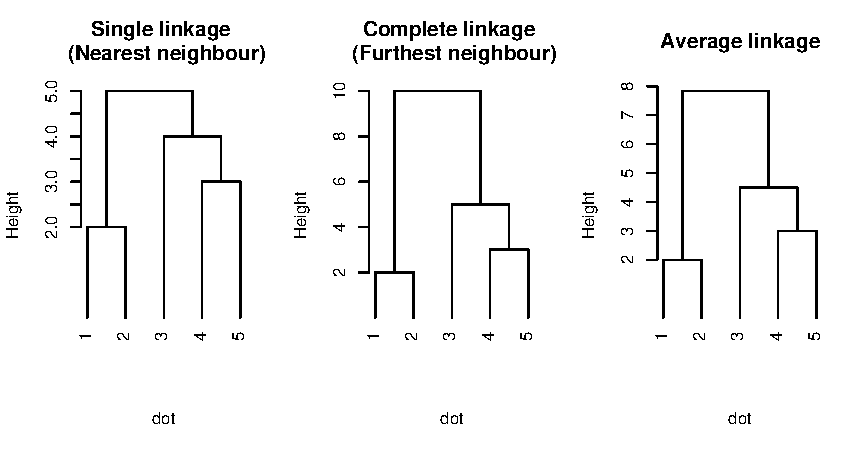
\includegraphics[width = 0.7\textwidth]{images/democlust}
\caption{Dendrograms from three basic cluster methods}
\label{simpleclust}
\end{center}
\end{figure}

%\begin{itemize}
%\item Ward's minimum variance method aims at finding compact, spherical clusters. 
%\item Complete linkage method finds similar clusters. 
%\item The single linkage method (which is closely related to the minimal spanning tree) adopts ``friends of friends'' clustering strategy. 
%\item Other methods are somewhere between single and complete link methods. 
%\end{itemize}

\subsection{Alternative methods for hierarchical cluster analysis}
\label{othermethods}

Given that cluster ``analysis'' is essentially an algorithmically guided exploratory data analysis it is perhaps no surprise, firstly that there have been many other methods proposed and secondly that there have been attempts to generalise the algorithm.   \cite{Lance+Williams:1966,Lance+Williams:1967} proposed a general recurrence formula which gives the distance between a newly amalgated group $C_{k} \bigcup C_{l}$ and some other group $C_{m}$:

\begin{equation}
d_{C_{k} \bigcup C_{l}, C_{m}} = \alpha_{l} d(C_{k}, C_{l}) + \alpha_{m} d(C_{k}, C_{m}) + \beta d(C_{k}, C_{l}) + \gamma \lvert d(C_{k}, C_{m}) -  d(C_{l}, C_{m})\rvert 
\end{equation}
where $d_{C_{k} \bigcup C_{l}, C_{m}}$ is the distance between a cluster $C_{k}$ and the merging of two groups  $C_{l}$ and $C_{m}$.   The parameters are constrained such that $\alpha_{l} + \alpha_{m} + \beta = 1$, $\alpha_{l} = \alpha_{m}$, $\beta < 1$ and $\gamma = 0$.   Using these schema, a number of established agglomerative strategies can be expressed as follows:
\begin{tabular}{lrrrr}
Method & \R call &  $\alpha_{k}$ & $\beta$ & $\gamma$ \\
\hline
Single link (nearest neighbour) & \verb+method = "single"+ & $\frac{1}{2}$ & 0 & $-\frac{1}{2}$ \\
Complete link (furthest neighbour) &  \verb+method = "complete"+ & $\frac{1}{2}$ & 0 & $\frac{1}{2}$ \\
Group average link &  \verb+method = "average"+ & $N_{l}|(N_{l} + N_{m})$ & 0 & 0\\
Weighted average link &  \verb+method = "mcquitty"+ & $\frac{1}{2}$ & 0 & 0 \\
Centroid &   \verb+method = "centroid"+ & $N_{l}|(N_{l} + N_{m})$ &  $- N_{l} N_{m}|(N_{l} + N_{m})^2$ & 0\\
%Sum of squares &  \verb+method = ""+ &  $(N_{i} + N_{K})|(N_{i} + N_{j} + N_{k})$ & $-(N_{K} + N_{k})|(N_{i} + N_{j} + N_{K})$
Incremental sum of squares &  \verb+method = "ward"+ & $\frac{N_{k} + N_{m}}{N_{k} + N_{l} + N_{m}}$ &  
$\frac{N_{k} + N_{l}}{N_{k} + N_{l} + N_{m}}$ & 0 \\
Median &  \verb+method = "median"+ & $\frac{1}{2}$ & $-\frac{1}{4}$ & 0\\
%Flexible & $\frac{1}{2}(1-\beta)$ & $\beta(<1)$ & 0\\
\end{tabular}
where $N_{k}, N_{l}\ \mbox{and}\ N_{m}$ are the cluster sizes when $C_{k}$ is joined to the other two clusters considered.

This formula facilitates the use of a number of clustering approaches.   \cite{Ward:1963} proposed a method in which clustering proceeds by selecting those merges which minimise the error sum of squares.   If we consider the cluster specific error sum of squares:
\begin{displaymath}
ESS_{k} = \sum_{i+1}^{n_{k}} \sum_{j=1}^{p} (x_{ki,j} - \bar{\boldsymbol{x}}_{k,j})^{2}
\end{displaymath}
where $ \bar{\boldsymbol{x}}_{k,j}$ is the mean of cluster $k$ with respect to variable $j$ and $x_{ki,j}$ is the value of $j$ for each object $i$ in cluster $k$.   The total error sum of squares is therefore given by $\sum_{k=1}^{K} ESS_{k}$ for all clusters $k$.   This method tends to give spherical clusters, whether that is a reasonable solution to find or not.

 Centroid clustering involves merging clusters with the most similar mean vectors; there is a subtle variation on a theme in which the centroid calculation is weighted.   Whilst the calculations underlying these methods tend to use Euclidean distance (to facilitate interpretation in terms of the raw data) that is not compulsory.   There is therefore some quite unsubtle interaction between choice of distance measure and choice of clustering algorithm which provides vast room for ambiguity in conducting cluster analysis.


\subsection{Problems with hierarchical cluster analysis}

A number of problems have been recognised with hierarchical cluster analysis.   Single, complete and average linkage as well as Ward's method have the potential for reversals in the dendrogram; single and complete linkage impose a monotonicity requirement.   One particular problem with single link clustering is ``chaining'', we could illustrate this as follows:
\singlespacing
\begin{verbatim}
x <- rbind(mvrnorm(30, c(0,0), sigma), 
  mvrnorm(30, c(8,8), sigma), 
  cbind(seq(0,8, by = 0.4), seq(0,8, by = 0.4) )
dot <- hclust(dist(x), method = "single")
par(mfrow = c(1,2))
plot(dot)
plot(x, pch = cutree(dot, k = 2))
\end{verbatim}
\onehalfspacing


\begin{figure}
\begin{center}
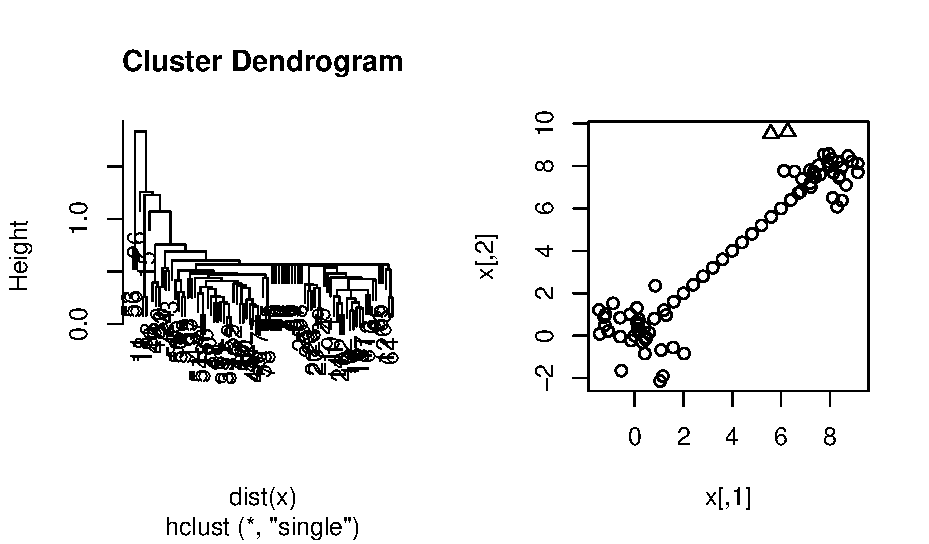
\includegraphics[width = 0.7\textwidth]{images/chaining}
\caption{Demonstration of ``chaining'' with single link clustering}
\label{chaining}
\end{center}
\end{figure}


\subsection{Hierarchical clustering in \R}

A typical example of a cluster analysis was reported by \cite{Jolliffe+etal:1986}. To carry out hierarchical cluster analysis in \R, create a distance object from the data (\verb+USArrests.dist+), create a hierarchical clustering object from the distance matrix (\verb+USArrests.hclust+), and plot the results.   Here we have used manhattan distance and compete linkage.  You may like to see how much difference the alternatives make.

\singlespacing
\begin{verbatim}
> USArrests.dist <- dist(USArrests, method = "manhattan")
> USArrests.hclust <- hclust(USArrests.dist, method = "complete")
> plot(USArrests.hclust)
\end{verbatim}
\onehalfspacing

\begin{figure}
\begin{center}
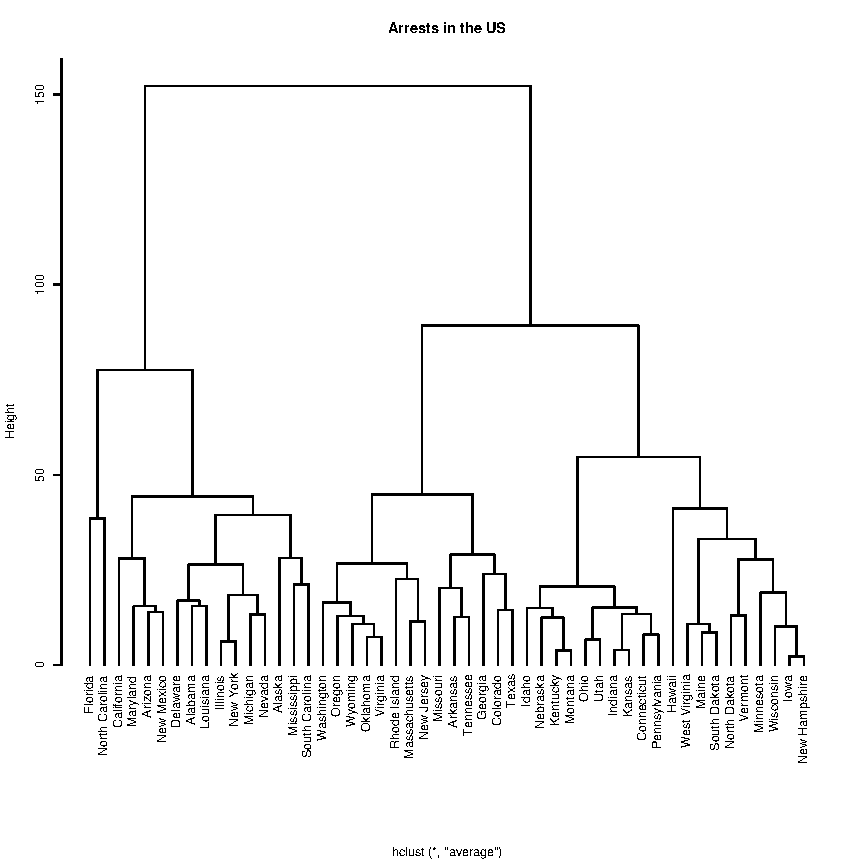
\includegraphics{images/hclust}
\caption{Dendrogram following complete linkage cluster analysis of US Arrests data}
\label{hclust}
\end{center}
\end{figure}

For comparison with other results, we may want to ``cut'' the dendrogram at a point which gives us a certain number of classes.   Here, we will cut the dendrogram fairly high up, and look at a possible five group structure.   In the following code, we use cutree to find the five groups, and produce draftsman plot with colours / symbols altering according to which of the five groups we think the state may belong to.

\singlespacing
\begin{verbatim}
> hc.class <- cutree(USArrests.hclust, k =5)
> plot(USArrests, col = hc.class, pch = hc.class)
\end{verbatim}
\onehalfspacing

An agreement is where both objects have a one in each position.   $b$ and $c$ denote the two possibly disagreements.

\section{Cophenetic Correlation}

The cophenetic correlation can be used as some kind of measure of the goodness of fit of a particular dendrogram.

\begin{equation}
\rho_{Cophenetic} = \frac{\sum_{i=1, j=1, i <j}^{n} (d_{ij} - \bar{d})(h_{ij} - \bar{h})}{
\left(\sum_{i=1, j=1, i <j}^{n} (d_{ij} - \bar{d})^{2}(h_{ij} - \bar{h})^{2} \right)^{0.5}}
\end{equation}

\singlespacing
\begin{verbatim}
> d1 <- dist(USArrests)
> h1 <- hclust(d1)
> d2 <- cophenetic(h1)
> cor(d1, d2)
[1] 0.7636926
> h1 <- hclust(d1, method = "single")
> d2 <- cophenetic(h1)
> cor(d1, d2)
[1] 0.5702505
\end{verbatim}
\onehalfspacing

So it is easy to obtain a measure of the cophenetic correlation, it is less clear what it means.   Certainly a value below 0.6 implies that there has been some distortion in the dendrogram.

\section{Divisive hierarchical clustering}
\label{aggclust}

Divisive clustering reverses the approach taken above.   Here, we start with one large cluster of all $n$ objects, and split until each object is unique. 
[page 90] \cite{Gordon:1999} argues that divisive clustering is not likely to lead to optimal divisions in the data.   Arguably the more succesful methods are monothetic and split on one variable at each stage (see \verb+mona()+ for an R example which works with binary data).      

\cite{MacNaughton-Smith+etal:1964} proposed one divisive method which has seen some use.   \cite{Kaufman+Rousseeuw:1989} liken this to splintering within a political party, where one person leaves and attracts the most like-minded people and have provided the \verb+diana()+ routine which facilitates this form of clustering.   


To identify the ``splinter'', the object with the largest average dissmilarity to all other objects is selected.   Then the dissimilarities are recalculated, and any objects who are closer to the splinter than to their original group are reclassified.   Average dissimilaries can then be recalculated.


At each subsequent step of the algorithm, the cluster $C$ with the largest diameter is selected:

\begin{displaymath}
diam(C) = max_{i,j \in C} d(i,j)
\end{displaymath}

This diameter is represented as the ``height'' in the dendrogram and the banner plot.

Then $C$ is split into two subclusters, initially $A=C$ and $B=\emptyset$.   For each objects in $A$, calculate the average dissimilarity to all other objects in $A$, the object with the largest distance is moved to $B$.   This step is repeated until there are $n$ clusters. 



\singlespacing
\begin{verbatim}
USArrests.dist <- dist(USArrests)
library(cluster)
USArrests.diana <- diana(USArrests.dist)
par(mfrow = c(1,2), oma = c(0,0,2,0))
plot(USArrests.diana, which = 2, cex = 0.6, 
main = "Dendrogram", xlab = "")
plot(USArrests.diana, which = 1, main = "Banner plot", 
nmax.lab = 50, cex.axis = 0.6, max.strlen = 12)
mtext("Divisive clustering of USArrests", outer = TRUE)
\end{verbatim}
\onehalfspacing




\begin{figure}
\begin{center}
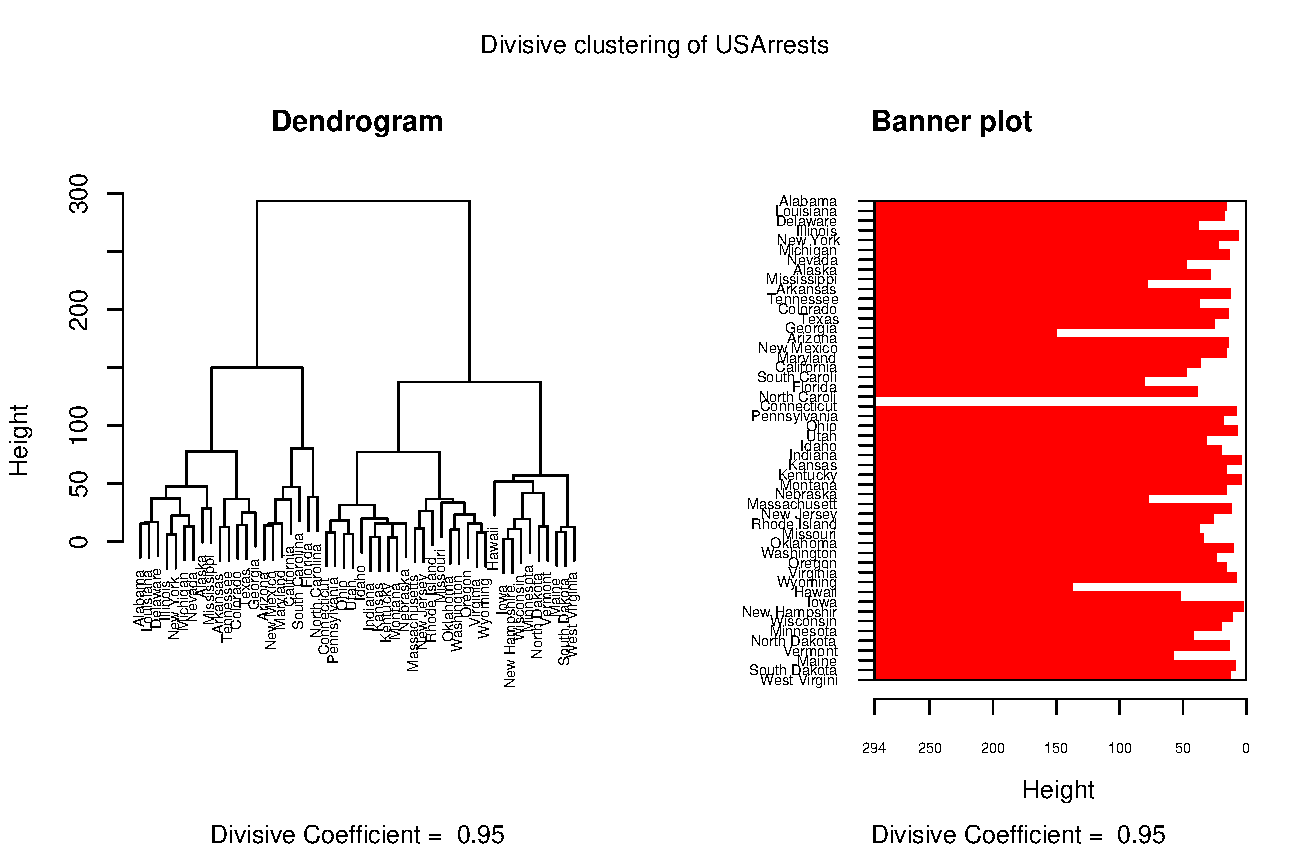
\includegraphics[width = 0.8\textwidth]{images/diana}
\caption{Divisive clustering of USArrests data, dendrogram and bannerplot}
\label{diana}
\end{center}
\end{figure}


\section{K-means clustering}
\label{kmclust}

This is a rather different method of clustering, aimed at finding ``more homogenous'' subgroups within the data.   We specify at the start how many clusters we are looking for, and ideally provide some clue as to what might be in those clusters.

The technique was perhaps first proposed by \cite{Lloyd:1957} and somewhat codified by \cite{Forgy:1965}, early developments were also reported by \cite{MacQueen:1967}, although the default S-Plus algorithm was developed by \cite{Hartigan+Wong:1979}.   There is some confusion as to whether \emph{k-means} refers to a particular technique or a particular algorithm.

Given a number of $k$ starting points, the data are classified, the centroids recalculated and the process iterates until stable.

We could attempt to demonstrate this with the following function

\singlespacing
\begin{verbatim}
step <- function(X, mu1, mu2){
## classify according to current seed point (expectation step)
one <- sqrt(rowSums((X - t(t(t(mu1)) %*% t(ones)))^2))
two <- sqrt(rowSums((X - t(t(t(mu2)) %*% t(ones)))^2))
plot(x,y, col = 1 + as.numeric(one < two), pch = 16, xlim = xlims, ylim = ylims )
legend("topright", pch = c(16,16,2,3), col = c("red", "black"), legend = c("Group1", "Group2", "Seed 1", "Seed 2" ), cex = 0.5)
points(rbind(seed$mu1, seed$mu2), pch = c(2,3), col = c("red", "black"))
fixed <- (mu1 + mu2)/2
slope <- -(mu1[1] - mu2[1])/(mu1[2] - mu2[2])
abline(c(fixed[2] - slope * fixed[1], slope))

## calculate new seed points (maximisation step)
mu1 <- colMeans(X[one < two,])
mu2 <- colMeans(X[one >= two,])
return(seed = list(mu1 = mu1, mu2 = mu2))
}
\end{verbatim}
\onehalfspacing

And set up with:

\singlespacing
\begin{verbatim}
## simulate two clusters of data
x <- c(rnorm(20,0,1), rnorm(20,4,1))
y <- c(rnorm(20,0,1), rnorm(20,4,1))
X <- cbind(x,y)
ones <- matrix(1, dim(X)[1],1)

## set up some parameters for plotting
xlims <- c(min(x), max(x)) * 1.3
ylims <- c(min(y), max(y)) * 1.3

## plot the data
par(mfrow = c(2,2))
plot(X, xlim = xlims, ylim = ylims)

## And add some very silly seed points
mu1 <- c(0,6)
mu2 <- c(5,-2)
seed <- list(mu1 = mu1, mu2 = mu2)
points(rbind(seed$mu1, seed$mu2), pch = c(2,3),col = c("red", "black"))
legend("topright", pch = c(1,2,3), col = c("black", "red", "black"), legend = c("Data", "Seed 1", "Seed 2" ), cex = 0.5)
##mtext(paste("Seed points: \n Group 1 ", formatC(seed[[1]],2), "Group 2 ", formatC(seed[[2]],2)))

seed <- step(X, seed$mu1, seed$mu2)
seed <- step(X, seed$mu1, seed$mu2)
seed <- step(X, seed$mu1, seed$mu2)
\end{verbatim}
\onehalfspacing

\begin{figure}
\begin{center}
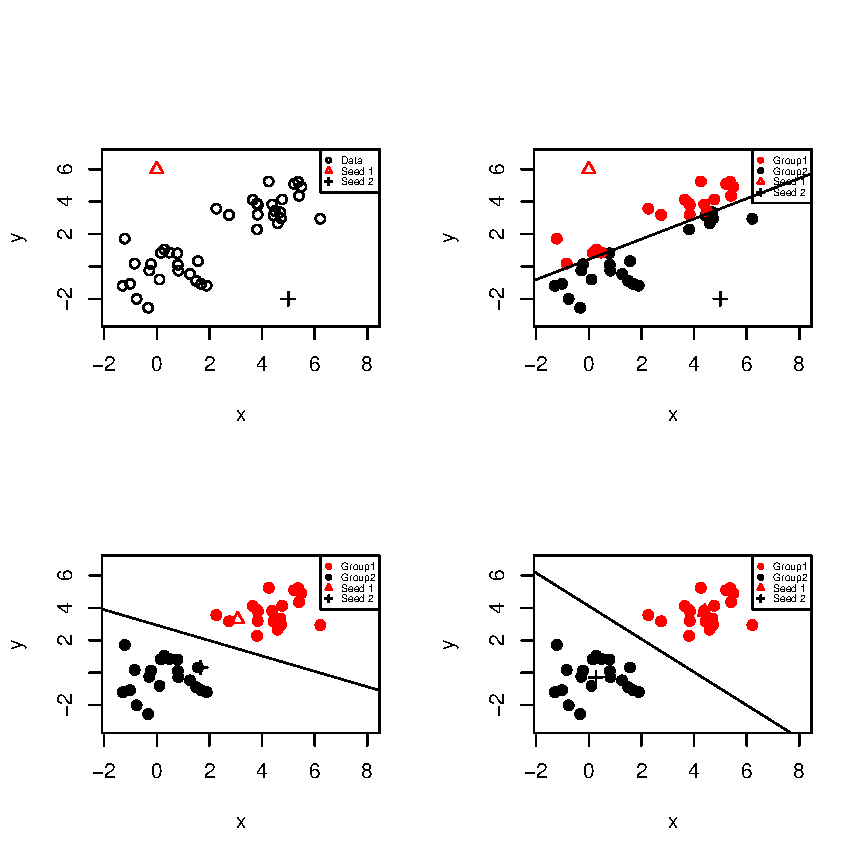
\includegraphics[width = 0.7\textwidth]{images/kmeansdemo}
\label{kmeansdemo}
\caption{Demonstration of kmeans algorithm, points are classified according to seed, then position of seed is recalculated}
\end{center}
\end{figure}

Having illustrated the basic principles it is quite easy to run the analysis:

\singlespacing
\begin{verbatim}
> US.km <- kmeans(USArrests, centers = 2)
> plot(USArrests, col = US.km$cluster, pch = US.km$cluster) ## not shown
> plot(prcomp(USArrests, center = TRUE)$x[,c(1,2)], 
col = US.km$cluster, pch = US.km$cluster)
 
\end{verbatim}
\onehalfspacing
For interest, we will compare the $k$-means solution with the \verb+diana()+ classification: 

\singlespacing
\begin{verbatim}
 kmclass <- as.vector(US.km$cluster)
> diana.class <- cutree(USArrests.diana, k = 2)
> xtabs(~kmclass + diana.class)
       diana.class
kmclass  1  2
      1  0 29
      2 21  0
\end{verbatim}
\onehalfspacing

So in this particular example, there is good agreement that there may be two clusters in the data.

\begin{figure}
\begin{center}
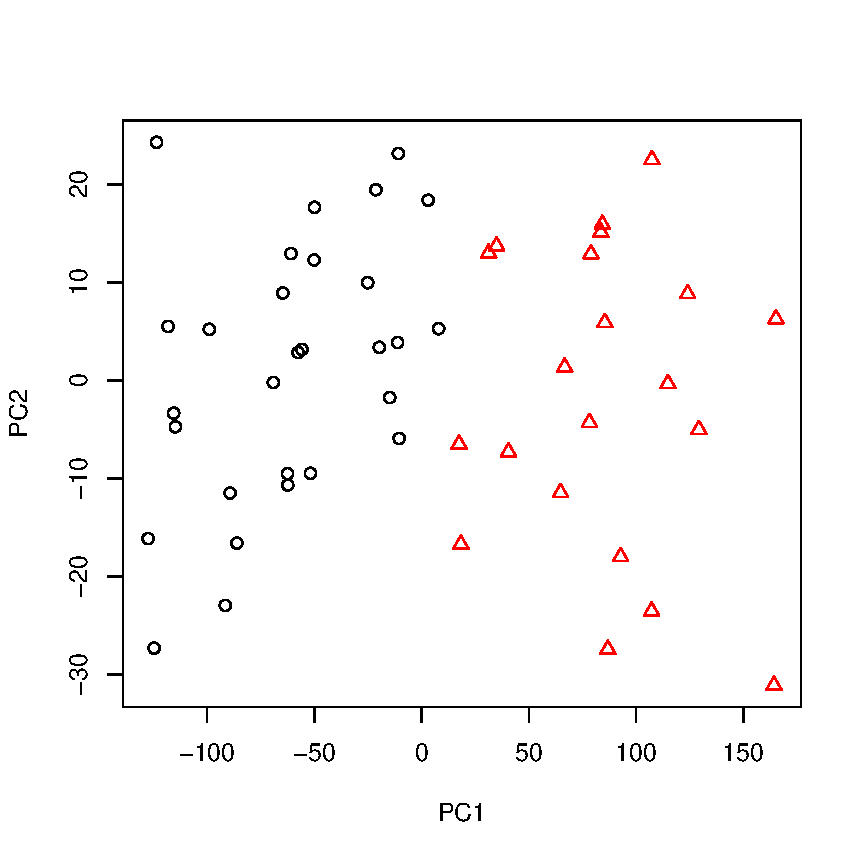
\includegraphics[width = 0.6\textwidth]{images/km2classpca}
\caption{Scatterplot of original variables denoting cluster membership for $k=2$ means clustering}
\label{hclust}
\end{center}
\end{figure}


\subsection{Partitioning around medoids}

This approach to clustering is laid out in \cite{Kaufman+Rousseeuw:1989}, and the S-PLUS implementation is very well described in \cite{Struyf+etal:1997}.   The procedure is to find $k$ \emph{representative objects} called medoids in such a way that the total dissimilarity of all objects to their nearest medoids is minimised.   One side-effect of this approach is that a data entity is identifed as a \emph{representative object} which may facilitate description rather better than a non-existing group centroid.   In other words, we identify objects that ``best'' represent their groups.   This is quite simple to do in \R, we can supply either the data matrix or a distance matrix to \verb+pam()+, below we supply the data:
\singlespacing
\begin{verbatim}
> USArrests.pam <- pam(USArrests, k = 2)
> par(mfrow = c(1,2))
> plot(USArrests.pam)
> USArrest.pam$medoids
         Murder Assault UrbanPop Rape
Michigan   12.1     255       74 35.1
Kansas      6.0     115       66 18.0
\end{verbatim}
\onehalfspacing
and it can be seen that Michigan and Kansas are in some sense the best representative examples of each of the two groups we have chosen to investigate.   The \verb+plot()+ method applied to pam objects produces a $2 \times 2$ scatterplot of the first two principal components identifying group memberships and superimposing ellipses as well as a silhouette.

\begin{figure}
\begin{center}
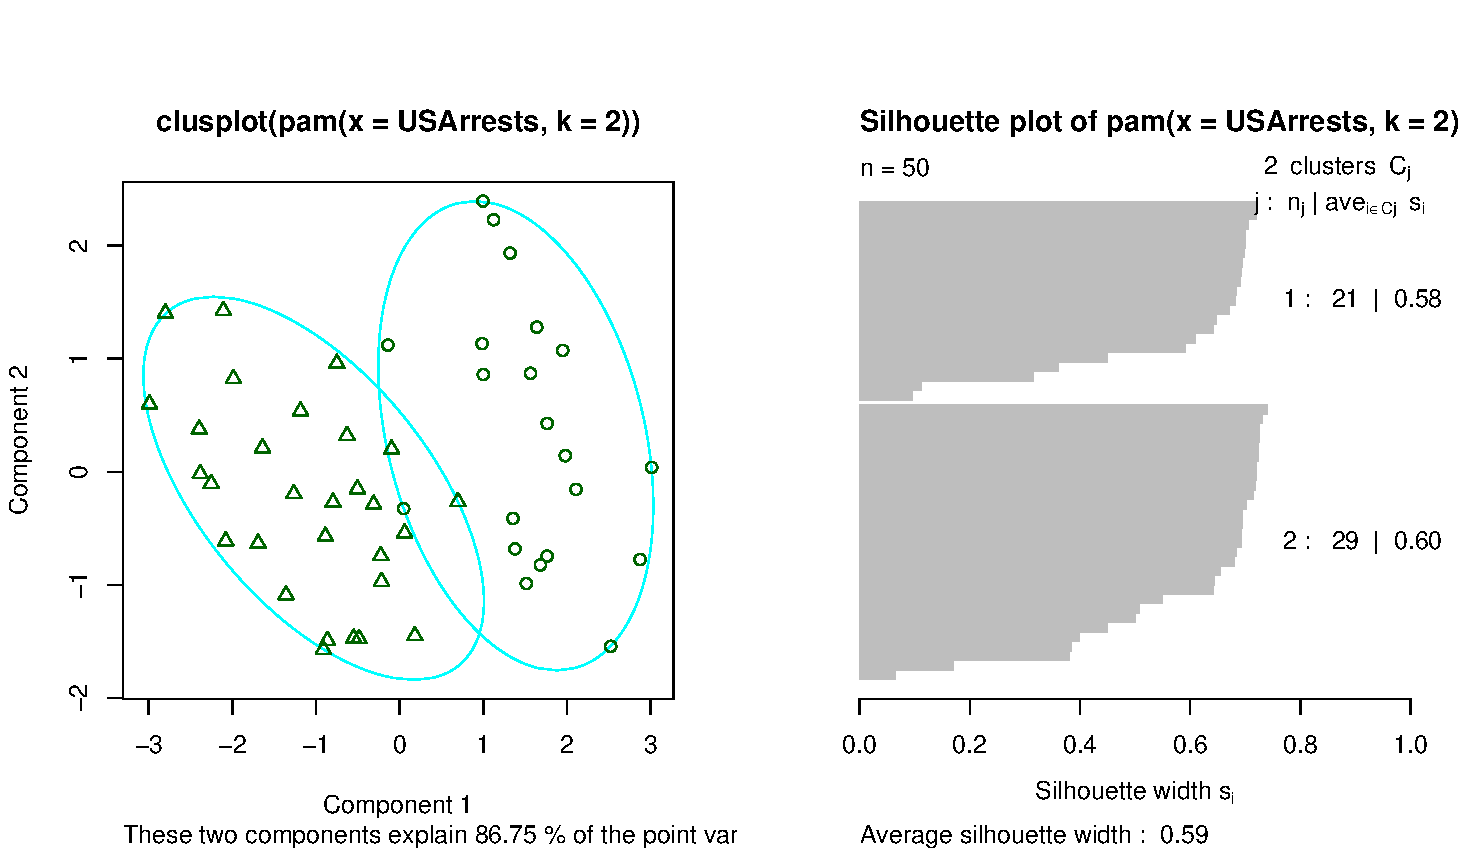
\includegraphics[width = 0.8\textwidth]{images/pam}
\caption{Partitioning around medoids}
\label{pam}
\end{center}
\end{figure}

With minor modification, this is a tractable algorithm for large datasets.   A wrapper, \verb+clara()+ has been written which makes partitioning around mediods available for a wide range of datasets.

\subsection{Hybrid Algorithms}

There have been a number of proposals in the literature recently for hybrid algrithms.   We consider HOPACH, essentially it is a divisive algorithm, but at each stage a merging step is incorporated to bring together similar clusters (which may be on different branches of the tree).  Again, this method produces medoids, in this case 13 were identified.

\singlespacing
\begin{verbatim}
> library(hopach)
> USArrests.hopach <- hopach(USArrests)
> row.names(USArrests)[USArrests.hopach$clustering$medoids]
 [1] "Mississippi"   "Alaska"        "New Mexico"    "Michigan"     
 [5] "California"    "Illinois"      "Missouri"      "West Virginia"
 [9] "Rhode Island"  "Nebraska"      "New Hampshire" "Wisconsin"    
[13] "Hawaii"     
> dplot(dist(USArrests), us, labels = row.names(USArrests), main = "HOPACH of USArrests")
\end{verbatim}
\onehalfspacing

The \verb+dplot()+ method requires input of a distnce matrix and produces a heatmap of the distances ordered by the cluster structure.   Silhouette plots are also available, and further plot methodology is available from programs external to \R.

\begin{figure}
\begin{center}
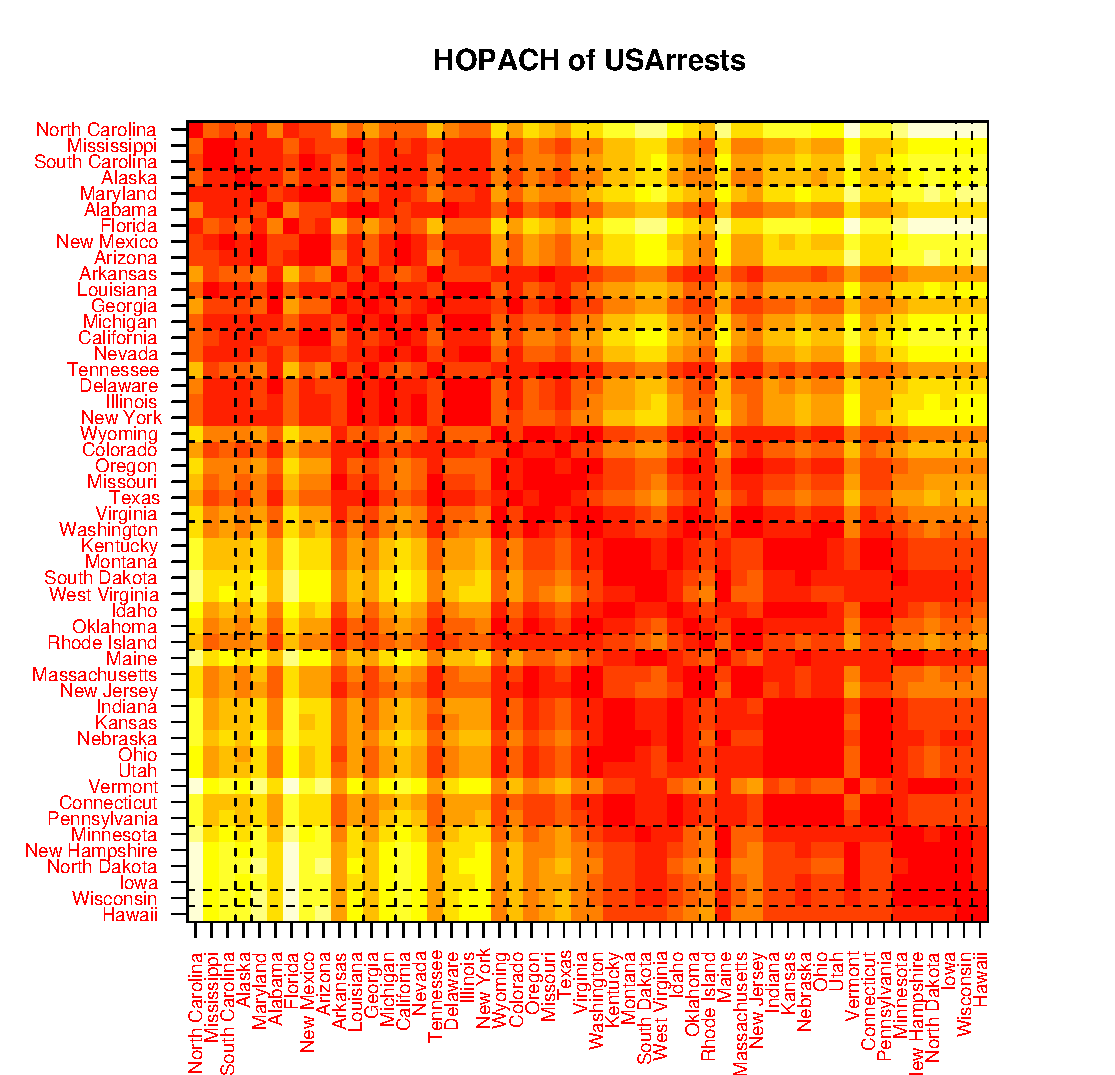
\includegraphics[width = 0.7\textwidth]{images/hopach}
\caption{Heatmap of distances organised according to output of HOPACH with cluster groups denoted by dashed lines}
\label{hopach}
\end{center}
\end{figure}

\section{K-centroids}

More recent proposals in the literature have tried to remove the dependency on algorithmic dependency.   I need to add something on this shortly.



\section{Further information}

It is worth repeating that ``cluster analysis'' is a poorly delimited set of methods for unsupervised classification.   Obvious omissions include fuzzy analysis (where we accept some uncertainty in group assignments), monothetic analysis (where we split based on binary variables one at a time).   All these merit further consideration.   However, it is acknowledged that the greatest omission at present is in terms of mixture modelling, much more comprehensive information is available in \cite{McLachlan+Peel:2000}, some coverage is also given in \cite{Flury:1997}.



%%% Local Variables: ***
%%% mode:latex ***
%%% TeX-master: "../book.tex"  ***
%%% End: ***